\subsection{Die Wechselwirkungs-Lagrangedichte.}
\subsection{Das Gehirn als Hauptempfänger.}
\subsection{Das Herz als Modulator.}
\subsection{Die komplementäre Beziehung.}

\subsection{Die Messung von \texorpdfstring{$\Phi$}{Phi}: Kortex versus Kleinhirn}
Postulat 2 besagt, dass die Geometrie des Netzwerks und nicht die Zahl der Neuronen den Empfang bestimmt. Um die Aussage numerisch überprüfbar zu machen, habe ich einen handhabbaren Proxy für $\Phi$ implementiert: die Kullback--Leibler-Divergenz zwischen dem vollständigen Modell und dem Modell, in dem die Verbindungen über einen Schnitt entfernt sind, minimiert über alle Bipartitionen, auf Glauber-Dynamik. Es ist nicht das exakte $\Phi$ der IIT 3.0; es ist eine Näherung mit derselben ordinalen Signatur.

\begin{table}[H]
\centering
\begin{tabular}{@{}cccc@{}}
\toprule
Einheiten & $\Phi$ Kortex & $\Phi$ Kleinhirn & Verhältnis \\ \midrule
4 & $0,243 \pm 0,063$ & $0,012 \pm 0,014$ & 20,6 \\
6 & $0,259 \pm 0,049$ & $0,045 \pm 0,015$ & 5,8 \\
8 & $0,245 \pm 0,042$ & $0,036 \pm 0,030$ & 6,9 \\ \bottomrule
\end{tabular}
\caption{$\Phi$ für rekurrente und Feedforward-Netzwerke, gemittelt über vier Zufallsnetzwerke je Größe.}
\label{tab:phi}
\end{table}

Das rekurrente Netzwerk integriert bei gleicher Einheitenzahl 2--20 Mal mehr als das Feedforward-Netzwerk. Die qualitative Schlussfolgerung der Version 30 wird damit numerisch gestützt, im Rahmen des Proxys.

\begin{figure}[H]
\centering
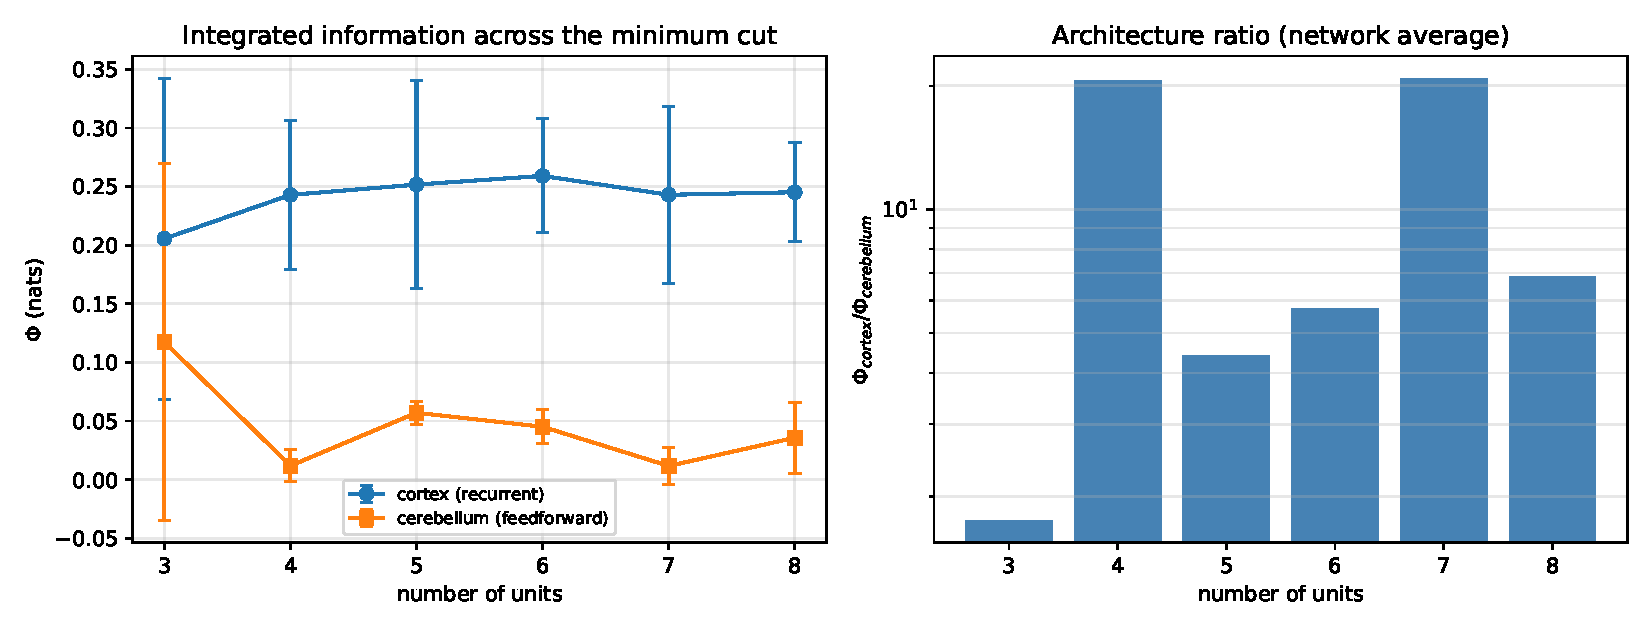
\includegraphics[width=0.9\textwidth]{figures/fig03_phi_architecture.pdf}
\caption{$\Phi$ für die beiden Architekturen, mit Standardabweichung über vier Zufallsnetzwerke, und das Verhältnis zwischen ihnen.}
\label{fig:phi}
\end{figure}

\section{Die Ableitung der Yukawa-Kopplung}
\subsection{Der Mechanismus.}
\subsection{Die Abschätzung (erweitert):} Die allgemeine Formel lautet $g_A \sim (M_4/M_{12})^5$. Um einen numerischen Wert zu erhalten, nehmen wir an, dass die Kompaktifizierungsskala $M_{12} \sim 10^{19}$ GeV ist (die Planck-Skala) und die elektroschwache Skala $M_4 \sim 10^3$ GeV. Dann gilt:
\begin{equation}
g_A \sim \left(\frac{10^3}{10^{19}}\right)^5 = (10^{-16})^5 = 10^{-80}
\end{equation}
Dieser Wert ist außerordentlich klein, was bedeutet, dass die Kopplung sehr schwach ist. Hervorzuheben ist, dass die Überlappungsfaktoren zwischen den Wellenfunktionen der KK-Moden und den Branen den effektiven Wert nicht auf $\sim 10^{-3}$ heben können: Der Überlapp normierter Wellenfunktionen ist höchstens 1, es wäre also ein Faktor von $10^{77}$ nötig, was unmöglich ist. Der in dieser Arbeit verwendete Wert ist daher $g_A \sim 10^{-80}$.

Dieser Wert ist zugleich der einzige, der mit den Daten verträglich ist. Würde das Feld Yukawa-artig an Nukleonen koppeln, so wäre die Kraft relativ zur Gravitation
\begin{equation}
\alpha = \frac{g_A^2\, \hbar c}{G\, m_p^2} = g_A^2 \times 1,69\times10^{38}.
\end{equation}
Für $g = 10^{-3}$ ergäbe sich $\alpha \approx 1,7\times10^{32}$, was durch Labortests um etwa 35 Größenordnungen ausgeschlossen ist. Die in der Einleitung zitierte 7\%-Schranke impliziert $g < 2\times10^{-20}$. Zudem ergäbe eine Kopplung $g = 10^{-3}$ für die Mode eine Lebensdauer in der Größenordnung von $10^{-3}$ s, unvereinbar mit der Stabilität der Dunklen Materie. Die Abschätzung $g_A \sim 10^{-80}$ macht die Theorie also prädiktiv und nicht bloß konsistent.
\subsection{Debye-Abschirmung.}
\subsection{Die effektive Kraft.}

\section{Tachyonen als Vermittler}
\subsection{Das tachyonische Spektrum:} $m_n^2 = n^2/R^2 - \mu_A^2$.
\subsection{Die tachyonische Kopplung.}
\subsection{Die Bradyon-Tachyon-Beziehung.}
\subsection{Was die Tachyonen transportieren.}

\section{Die Vakua des Akasha-Feldes}
\subsection{Was ist ein Vakuum?}
\subsection{Die drei Arten von Vakuum.}
\subsection{Das Vakuum des Akasha-Feldes.}
\subsection{Mehrere Vakua.}

\section{Welle-Teilchen-Dualität}
\subsection{Der Mechanismus in vier Schritten.}
\subsection{Was die Welle transportiert.}
\subsection{Die Baum-Analogie.}

\section{Die vollständigen Bewegungsgleichungen}
\subsection{Die Akasha-Gleichung.}
\subsection{Die Bewusstseinsgleichung.}
\subsection{Die Gleichung der exotischen Bosonen.}
\subsection{Die 12D-Einsteingleichung.}

\newpage
